%!TEX root = ../thesis.tex
%*******************************************************************************
%*********************************** First Chapter *****************************
%*******************************************************************************

\chapter{Introduction}  %Title of the First Chapter

\ifpdf
    \graphicspath{{Chapter1/Figs/Raster/}{Chapter1/Figs/PDF/}{Chapter1/Figs/}}
\else
    \graphicspath{{Chapter1/Figs/Vector/}{Chapter1/Figs/}}
\fi


%********************************** %First Section  **************************************

\section{Problem Statement}

Deep Neural Networks (DNNs), are connectionist systems that learn to perform tasks by learning on examples without having a prior knowledge about the tasks. 
They easily scale to millions of data points and yet remain tractable to optimize with stochastic gradient descent.

Convolutional Neural Networks (CNNs), a variant of DNNs, have already surpassed human accuracy in the realm of image classification (e.g. \cite{he2016deep,simonyan2014very,krizhevsky2012imagenet}). Due to the capacity of CNNs to fit on a wide diversity of non-linear data points, they require large amount of training data. This often makes CNNs and Neural Networks in general, prone to overfitting on small datasets. The model tends to fit well to the training data, but are not predictive for new data. This often makes the Neural Networks incapable of correctly assessing the uncertainty in the training data and hence leads to overly confident decisions about the correct class, prediction or action.

Various regularization techniques for controlling overfitting are used in practice namely  early stopping, weight decay, L1, L2 regularizations and currently the most popular and empirically effective technique being \emph{dropout}~\cite{hinton2012improving}. 

We will address both of these concerns by using Bayesian learning to add a measure for uncertainty and regularization in their predictions. 

\section{How to tackle the problem}

Deep Neural Networks have been successfully applied to many domains, including sensitive domains like health-care, security, fraudulent transactions and many more. However, from a probability theory perspective, it is unjustifiable to use single point-estimates as weights to base any classification on.
On the other hand, Bayesian neural networks (NNs) are more robust to over-fittings, and can easily learn from small datasets. Bayesian approach further offers uncertainty estimates via its parameters in form of probability distributions (see Figure \ref{fig:Scalar_Bayesian_Distribution}). At the same time, by using a prior probability distribution to integrate out the parameters, we compute the average across many models during training, which gives a regularization effect to the network, thus preventing overfitting.


Bayesian posterior inference over the neural network parameters is a theoretically attractive method for controlling overfitting; however, modelling a distribution over the kernels (also known as filters) of a CNN has never been attempted successfully before, perhaps because of the vast number of parameters and extremely large models commonly used in practical applications.

Even with a small number of parameters, inferring model posterior in a Bayesian NN is a difficult task. Approximations to the model posterior are often used instead, with variational inference being a popular approach. In this approach one would model the posterior using a simple \textit{variational} distribution such as a Gaussian, and try to fit the distribution's parameters to be as close as possible to the true posterior. This is done by minimising the Kullback-Leibler divergence from the true posterior. Many have followed this approach in the past for standard NN models \citep{hinton1993keeping,barber1998ensemble,graves2011practical,blundell2015weight}.
But the variational approach used to approximate the posterior in Bayesian NNs can be fairly computationally expensive -- the use of Gaussian approximating distributions increases the number of model parameters considerably, without increasing model capacity by much. \citet{blundell2015weight} for example use Gaussian distributions for Bayesian NN posterior approximation and have doubled the number of model parameters, yet report the same predictive performance as traditional approaches using dropout. This makes the approach unsuitable for use with CNNs as the increase in the number of parameters is too costly.

\begin{figure}[t]
\begin{center}
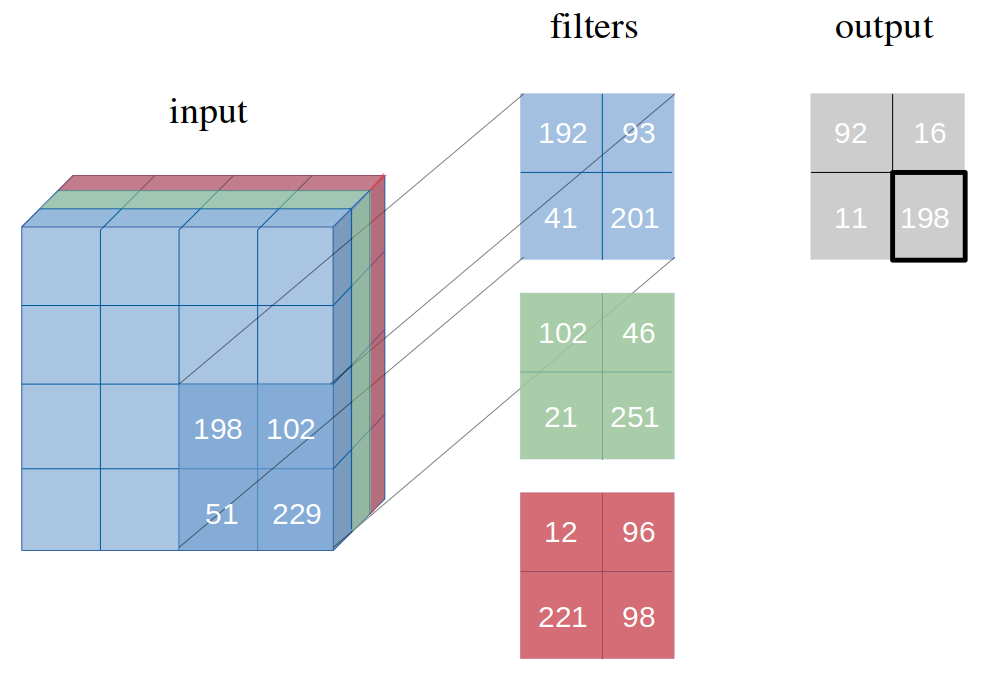
\includegraphics[height=.28\textheight]{Chapter1/Figs/filter_scalars.png}
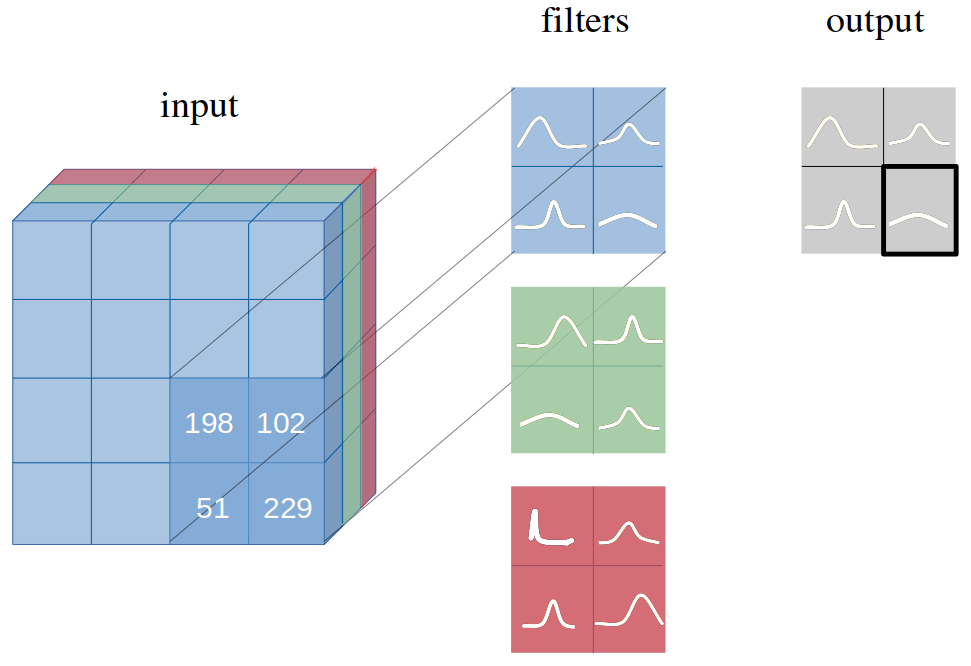
\includegraphics[height=.28\textheight]{Chapter1/Figs/CNNwithdist.png}
\label{fig:Scalar_Bayesian_Distribution}
\caption{Top: Each filter weight has a fixed value, as in the case of frequentist Convolutional Networks. Bottom: Each filter weight has a distribution, as in case of Bayesian Convolutional Networks.}
\end{center}
\end{figure}

\newline We build our Bayesian \ac{cnn} upon \textit{Bayes by Backprop} \cite{graves2011practical,blundell2015weight}. The exact Bayesian inference on the weights of a neural network is intractable as the number of parameters is very large and the functional form of a neural network does not lend itself to exact integration. So, we approximate the intractable true posterior probability distributions $p(w|\mathcal{D})$ with variational probability distributions $q_{\theta}(w|\mathcal{D})$, which comprise the properties of Gaussian distributions $\mu \in \mathbb{R}^d$ and $\sigma \in \mathbb{R}^d$, denoted $\mathcal{N}(\theta|\mu, \sigma^2)$, where $d$ is the total number of parameters defining a probability distribution. The shape of these Gaussian variational posterior probability distributions, determined by their variance $\sigma^2$, expresses an uncertainty estimation of every model parameter. \\ \\
\newline The main contributions of our work are as follows: 
\begin{enumerate}
    \item We present how \textit{Bayes by Backprop} can be efficiently applied to \acp{cnn}. We therefore introduce the idea of applying two convolutional operations, one for the mean and one for the variance.
    \item We show how the model learn richer representations and predictions from cheap model averaging.
    \item We empirically show that our proposed generic and reliable variational inference method for Bayesian \acp{cnn} can be applied to various \ac{cnn} architectures without any limitations on their performances. 
    \item We examine how to estimate the aleatoric and epistemic uncertainties and empirically show how the uncertainty can decrease, allowing the decisions made by the network to become more deterministic as the training accuracy increases. 
    \item We also empirically show how our method typically only doubles the number of parameters yet trains an infinite ensemble using unbiased Monte Carlo estimates of the gradients. 
\end{enumerate} 
This work builds on the foundations laid out by Blundell et al. \cite{blundell2015weight}, who introduced \textit{Bayes by Backprop} for feedforward neural networks. Together with the extension to recurrent neural networks, introduced by Fortunato et al. \cite{fortunato2017bayesian}, \textit{Bayes by Backprop} is now applicable on the three most frequently used types of neural networks, i.e., feedforward, recurrent, and convolutional neural networks.


\nomenclature[z-cif]{$CIF$}{Cauchy's Integral Formula}                                % first letter Z is for Acronyms 
\nomenclature[a-F]{$F$}{complex function}                                                   % first letter A is for Roman symbols
\nomenclature[g-p]{$\pi$}{ $\simeq 3.14\ldots$}                                             % first letter G is for Greek Symbols
\nomenclature[g-i]{$\iota$}{unit imaginary number $\sqrt{-1}$}                      % first letter G is for Greek Symbols
\nomenclature[g-g]{$\gamma$}{a simply closed curve on a complex plane}  % first letter G is for Greek Symbols
\nomenclature[x-i]{$\oint_\gamma$}{integration around a curve $\gamma$} % first letter X is for Other Symbols
\nomenclature[r-j]{$j$}{superscript index}                                                       % first letter R is for superscripts
\nomenclature[s-0]{$0$}{subscript index}                                                        % first letter S is for subscripts


%********************************** %Second Section  *************************************

\nomenclature[z-DEM]{DEM}{Discrete Element Method}
\nomenclature[z-FEM]{FEM}{Finite Element Method}
\nomenclature[z-PFEM]{PFEM}{Particle Finite Element Method}
\nomenclature[z-FVM]{FVM}{Finite Volume Method}
\nomenclature[z-BEM]{BEM}{Boundary Element Method}
\nomenclature[z-MPM]{MPM}{Material Point Method}
\nomenclature[z-LBM]{LBM}{Lattice Boltzmann Method}
\nomenclature[z-MRT]{MRT}{Multi-Relaxation 
Time}
\nomenclature[z-RVE]{RVE}{Representative Elemental Volume}
\nomenclature[z-GPU]{GPU}{Graphics Processing Unit}
\nomenclature[z-SH]{SH}{Savage Hutter}
\nomenclature[z-CFD]{CFD}{Computational Fluid Dynamics}
\nomenclature[z-LES]{LES}{Large Eddy Simulation}
\nomenclature[z-FLOP]{FLOP}{Floating Point Operations}
\nomenclature[z-ALU]{ALU}{Arithmetic Logic Unit}
\nomenclature[z-FPU]{FPU}{Floating Point Unit}
\nomenclature[z-SM]{SM}{Streaming Multiprocessors}
\nomenclature[z-PCI]{PCI}{Peripheral Component Interconnect}
\nomenclature[z-CK]{CK}{Carman - Kozeny}
\nomenclature[z-CD]{CD}{Contact Dynamics}
\nomenclature[z-DNS]{DNS}{Direct Numerical Simulation}
\nomenclature[z-EFG]{EFG}{Element-Free Galerkin}
\nomenclature[z-PIC]{PIC}{Particle-in-cell}
\nomenclature[z-USF]{USF}{Update Stress First}
\nomenclature[z-USL]{USL}{Update Stress Last}
\nomenclature[s-crit]{crit}{Critical state}
\nomenclature[z-DKT]{DKT}{Draft Kiss Tumble}
\nomenclature[z-PPC]{PPC}{Particles per cell}